\documentclass[runningheads]{llncs}

\usepackage[utf8]{inputenc}
\usepackage{graphicx}
\usepackage{mathpazo}
\usepackage{todonotes}
\usepackage{subcaption}
\usepackage{float}

% Todo commands

\newcommand{\todoin}[2][]{\todo[inline, color=blue!40, #1]{#2}}
\newcommand{\fixme}[2][]{\todo[color=yellow!40, #1]{#2}}
\newcommand{\fixmein}[2][]{\todo[inline, color=yellow!40, #1]{#2}}
\renewcommand{\arraystretch}{1.7}


% If you use the hyperref package, please uncomment the following line
% to display URLs in blue roman font according to Springer's eBook style:
% \renewcommand\UrlFont{\color{blue}\rmfamily}

\begin{document}

\title{Ant Colony Optimization algorithms \\
for the Permutation Flow Shop Problem with Weighted Tardiness}
\subtitle{}

\titlerunning{ACO algorithms for PFSP-WT}

\author{Hakim Boulahya \\
hboulahy@ulb.ac.be}

\authorrunning{H. Boulahya}

\institute{Université Libre de Bruxelles}

\maketitle

\begin{abstract}
In this article we present two implementations of Ant Colony Optimization metaheuristic algorithms for the
Permutation Flow Shop Problem with Weighted Tardiness minimization objective (PFSP-WT). We implement Ant Colony System and $\mathcal{MAX – MIN}$ Ant System and compare the results. The algorithms were extended using local search methods to improve local solutions, and provide better results. To reach better performance and tune parameters \texttt{irace},
an off-line automated parameters tuning tool, was used. We then conclude by analysis the results
and propose the best found algorithm to provide a good solution to the PFSP-WT problem.

\keywords{PFSP \and PFSP-WT \and ACO  \and ACS \and MMAS \and Ant Colony Optimization.}
\end{abstract}

\section{Introduction}

The PFSP-WT is the problem where jobs have to be schedule on a multi-machine setup. Let $\pi = (1, 2, ..., n)$ be a permutation of jobs that represents a schedule with $n$ the number of jobs. The interpretation of the schedule is as follow: all machine execute the job in the same orders defined in $\pi$. A job can only be executed if the previous job on the same machine is completed and if the execution of the same job in the previous machine is also completed. The objective of this problem it to minimize the total weigheted tardiness of jobs $\sum_{i=1}^{n}{w_i T_i}$, where $T_i = max(C_i - d_i, 0)$ represents the tardiness of job $i$ and $w_i$ the weight of job $i$. $C_i$ is the completion time of job $i$ in the last machine and $d_i$ the due date of job $i$. The completion time of job $i$ in machine $j$ is defined as follow:

\begin{equation}
  C_{i,j} = max(C_{i-1,j}, C_{i, j-1}) + p_{ij}
\end{equation}

where $p_{ij}$ represents the processing time of job $i$ on machine $j$. The completion time of the jobs in the first machine is the accumulation of processing times of all the jobs, where the completion time of the first job set to its processing time.

In the following sections, we described two Ant Colony Optimization (ACO) algorithms: Ant Colony System (ACS) and  $\mathcal{MAX – MIN}$ Ant System (MMAS) to solve this problem. We then describe two local search methods to enhance the algorithms. Finally we define the parameters and methodology used to test the implementation and analyse the results.

\section{Ant Colony Optimization algorithms for PFSP-WT}

\paragraph{}

In this section we define the representation of the solution and the different variables and methods use to implement ACS and MMAS. Both algorithms are implemented as follow: while the termination condition is not met, a number of ants will build a schedule, and only the best-iteration ant solution is kept if it is better than the global-best solution. The global-best solution is initialized as described in \ref{heuristic}.

\paragraph{}

A termination condition corresponds to a set of three sub-conditions: either the number of iterations is reach, number of steps is reached or a maximum set time has been reach. A step is the unit of measure that counts the number of schedules build by all the ants.


\paragraph{}

For the implementaion of ACS our work is inspired from the variables and methods studied by Den Besten et al. in \cite{den_besten_ant_2000}. They studied the PFSP-WT problem where only a single machine is taking into consideration. For MMAS, we extended the definition of the variables defined in \cite{stutzle_ant_1997} with the exhaustive description of ACO algorithms from the reference book of  Dr. Dorigo \cite{dorigo_ant_2004}, The objective function was also modified to minimize the total weigheted tardiness (where Stutzle minimize the makespan) as defined in \cite{den_besten_ant_2000}.

\subsection{Solution representation} For the PFSP-WT problem, a solution is a permutation of jobs $\pi = (1, 2, ..., n)$
that must be scheduled and executed.
The objective is to minimize the sum weighted tardiness
$\sum_{i=1}^{n}{w_i T_i}$ of a permutation of jobs.




\subsection{Schedule construction}
\paragraph{Remark}

When not specified $\tau_{ij}$ and $\eta_{ij}$ correspond to $\tau_{ij}(t)$ and $\eta_{ij}(t)$,
where $\tau_{ij}(t)$ is the pheromone trail of the job $i$ in position $j$ of the current schedule and $\eta_{ij}$ the heuristic desirabity of the trail.

\paragraph{}

An ant will build a schedule as follow: at first, the solution is empty. Then for all the positions the ant select with probability $q_0$ the unscheduled job $i$ for position $j$ that maximize $(\tau_{ij})^\alpha (\eta_{ij})^\beta$, that is:

\begin{equation}
\mathrm{argmax}_{unscheduled}(\tau_{ij})^\alpha (\eta_{ij})^\beta
\end{equation}

\paragraph{}

Otherwise, an ant explores with probabilibty $1 - q_0$ where the probability distribution to select an unscheduled job is:

\begin{equation}
p_{ij} = \frac{(\tau_{ij})^\alpha (\eta_{ij})^\beta}{\sum_{unscheduled}{(\tau_{ij})^\alpha (\eta_{ij})^\beta}}
\end{equation}

\subsection{Heuristic information}

\label{heuristic}

To initialize the solution and the heuristic information $\eta_{ij}$, the Earliest Due Date (EDD) heuristic was implemented \cite{den_besten_ant_2000}. This heuristic puts the initial solution in non-decreasing order of the due dates $d_i$ and initialize the heuristic information as $\eta_{ij} = 1/d_i$, where $\eta_{ij}$ is the heuristic information: when combined with $\tau_{ij}$
it is the desirabity of putting job $i$ in position $j$ \cite{den_besten_ant_2000}.





\subsection{Ant Colony System}

In addition of the construction defined in the previous section, ACS defined two methods to update the pheromones: global and local.

\subsubsection{Global Pheromone Trail Update}

\begin{equation}
\tau_{ij}(t+1) = (1 - \rho) \cdot \tau_{ij}(t) + \rho \cdot \Delta \tau_{ij}(t)
\end{equation}

where $\Delta \tau_{ij}(t)$ = $ 1 / T^{*}$ with $T^*$ the total weighted tardiness of the current solution and $\rho$ the parameter for trail evaporation.

\subsubsection{Local Pheromone Trail Update}

During schedule construction, each time an ant add a job $i$ in position $j$ the following update rule \cite{den_besten_ant_2000} is applied:

\begin{equation}
\tau_{ij} = (1 - \xi) \cdot \tau_{ij} + \xi \cdot \tau_{0}
\end{equation}

Where $0 < \xi \le 1$ and $\tau_0$ is set as the initial value of the pheromone trails set to $\tau_0 = 1 / (n \cdot T_{EDD})$ \cite{den_besten_ant_2000}, with $n$ is the number of jobs and
$T_{EDD}$ the total weighted tardiness of the solution generated by the heuristic $EDD$.

\subsection{$\mathcal{MAX – MIN}$ Ant System}


\subsubsection{Schedule construction}

$\mathcal{MAX – MIN}$ is set to always explore unscheduled jobs, that is $q_0 = 1$\fixme{This is wrong, it should be $q_0 = 0$ to always explore.}.


\subsubsection{Global Pheromone Trail Update}

\begin{equation}
\tau_{ij}(t+1) = (1 - \rho) \cdot \tau_{ij}(t) + \Delta \tau_{ij}(t)
\end{equation}

\subsubsection{Pheromone Trails Limits}

$\tau_{max}$ is set set to $1 / \rho T^*$ and upated at each iteration, each time a new
best-so-far is found.
$\tau_{min} = \tau_{max} / a$ where a is set to $5$ \cite{stutzle_ant_1997}. The trails are initialized to $\tau_{max}$.

\subsubsection{Pheromone Trails Initialization and Reinitialization}

If the algorithm after a number of iterations stagnate, then the
pheromone trails are reinitialized to $\tau_{max}$.

\subsection{Local search}

\label{localsearch}

\paragraph{}


To improve the performance and the results of the algorithms, local search was added. The method chosen to perform local search is by using \textit{insertion-moves} \cite{stutzle_ant_1997}. That is for all existing permutation $(i, j)$, where $i$ is the position where the job has to be removed and $j$ the position where the job has to be inserted with $i \neq j$. This local search is performs in $O(n^2)$.

\paragraph{}

Two mechanisms were implemented to perform local search: \textit{best-ant} and \textit{all-ant}. With \textit{best-ant} only the best-iteration ant is allowed to perform local search, this computes in $O(n^2)$ per iteration. With \textit{all-ant}, all ants perform local search at each iteration. \textit{all-ant} mechanism computes in $O(mn^2)$, where $m$ is the number of ants.

\section{Final Results}

\subsection{Methodology}

This section presents the results of the executions of the algorithms.
We show and compare the results of six algorithms: ACS, MMAS, ACS-LS-BEST, ACS-LS-ALL, MMAS-LS-BEST and MMAS-LS-ALL, where ACS and MMAS are the ACO algorithms without local search and the others are the respective algorithms with local search enabled using the method described in \ref{localsearch}. For example, MMAS-LS-BEST is MMAS with local search enabled where only the best-iteration ant performs local search.

\paragraph{Setup} To generate data, we executed ten runs of all six algorithms for each of the twenty instances \cite{taillard}  (1200 executions in total), with a budget of 30 seconds per execution. The experiments were run using an Intel(R) Xeon(R) E5-2620 CPU with 32 Cores and 64GB of RAM on CentOS 7.

\subsection{Parameter settings}

For setting the parameters, we used \texttt{irace} \cite{irace}.
We tuned the parameters listed in Table \ref{table:irace} with a maximum number of experiments
set to $200$. Note that $q_0$ and $\xi$ are not tuned for MMAS as there is only exploration and no local update in this algorithm.

\begin{table}[]
\centering
\begin{tabular}{ | l | l | c | c | c | c | c | c | c | }
  \hline
  Parameter    & Range          & ACS    & MMAS    & ACS-LS-BEST & ACS-LS-ALL & MMAS-LS-BEST & MMAS-LS-ALL \\
  \hline
  ants         & (5, 100)       & 41     & 28      & 5        &  93   & 34  & 87 \\
  \hline
  $\alpha$        & (0.00, 5.00)   & 2.56   & 3.88    & 2.83     &  3.69    &   4.41     & 0.34 \\
  \hline
  $\beta$         & (0.00, 10.00)  & 7.78   & 6.69    & 3.28     &  5.08     & 9.48      & 6.76 \\
  \hline
  $\rho$          & (0.01, 1.00)   & 0.32   & 0.53    & 0.61     &  0.05      &   0.41     & 0.7 \\
  \hline
  $\xi$          & (0.01, 1.00)   & 0.46    & 0.53    & 0.38     &  0.77     &       -      & - \\
  \hline
  $q_0$           & (0.0, 1.0)     & 0.07   & -       & 0.04     &  0.24    &       -      & - \\
  \hline

\end{tabular}
\caption{Parameters tuned and best configurations returned by \texttt{irace} for each algorithm}
\label{table:irace}
\end{table}

\subsection{Analysis}

\paragraph{}

In Table \ref{table:best}, the best total weighted tardiness for each instance returned by each algorithms is shown. As one can see algorithms with local search enabled always perform better. With those results, one would suggests that the preferred algorithm might depend on the instance itself. MMAS seems to performs better on instances with more jobs, where ACS is most of time better with instances with less jobs. Regarding the comparison between the different local search method described in \ref{localsearch}, \textit{best-ant} seems to always be a better choice compared to \textit{all-ant}. One could say that the fact that only the best ant is allowed to search locally, enables the algorithm to look for better solution faster.

\paragraph{}

Figure \ref{fig:ta_051} show the solutions quality and the convergence of the algorithms for an instance with 50 jobs where Figure \ref{fig:ta_090} show the corresping plots for an instance with 100 jobs. In both cases, the algorithms with \textit{best-ant} local search converge faster to better solutions, and the quality of the solution is often better.


\begin{table}[H]
  \centering
  \begin{tabular}{|l|l|l|l|l|l|l|}
  \hline
  Instance  & ACS \qquad     & MMAS    & ACS\_LS\_BEST & ACS\_LS\_ALL & MMAS\_LS\_BEST & MMAS\_LS\_ALL \\
  \hline
  DD\_Ta051 & 87021   & 87907   & 52055         & 70168        & \textbf{44847}          & 53427         \\
  \hline
  DD\_Ta053 & 108723  & 118469  & \textbf{61368}         & 77178        & 69128          & 74998         \\
  \hline
  DD\_Ta054 & 102680  & 107279  & \textbf{59899}         & 86431        & 60958          & 67105         \\
  \hline
  DD\_Ta055 & 73943   & 78490   & \textbf{32623}         & 61840        & 41799          & 41248         \\
  \hline
  DD\_Ta052 & 98254   & 104456  & 60866         & 79199        & \textbf{54697}          & 65945         \\
  \hline
  DD\_Ta056 & 70778   & 70824   & \textbf{35330}         & 65928        & 40988          & 51824         \\
  \hline
  DD\_Ta057 & 90580   & 98918   & \textbf{47534}         & 78845        & 48303          & 62596         \\
  \hline
  DD\_Ta058 & 85556   & 95524   & \textbf{57207}         & 86977        & 58272          & 72187         \\
  \hline
  DD\_Ta059 & 81253   & 83349   & 52033         & 68901        & \textbf{49384}          & 55720         \\
  \hline
  DD\_Ta060 & 146394  & 169210  & 117216        & 127819       & 117058         & \textbf{105088}        \\
  \hline
  DD\_Ta081 & 954686  & 958138  & 900036        & 955650       & 879685         & \textbf{881917}        \\
  \hline
  DD\_Ta082 & 859666  & 844413  & \textbf{766361}        & 842497       & 802836         & 805140        \\
  \hline
  DD\_Ta083 & 1068515 & 1059775 & 991420        & 1041605      & \textbf{980420}         & 1027187       \\
  \hline
  DD\_Ta084 & 1138753 & 1171783 & \textbf{1089303}       & 1139172      & 1103457        & 1139404       \\
  \hline
  DD\_Ta085 & 1062634 & 1082410 & 1005153       & 1077911      & 1000383        & \textbf{975061}        \\
  \hline
  DD\_Ta086 & 1060223 & 1092469 & 1042539       & 1035553      & \textbf{993250}         & 1039797       \\
  \hline
  DD\_Ta087 & 895045  & 926469  & 873978        & 915212       & \textbf{873015}         & 875673        \\
  \hline
  DD\_Ta088 & 1015562 & 1043175 & 991322        & 1008984      & \textbf{977752}         & 978800        \\
  \hline
  DD\_Ta089 & 1099690 & 1137683 & 1088799       & 1120113      & 1100444        & \textbf{1085154}       \\
  \hline
  DD\_Ta090 & 1040605 & 1060481 & 1001944       & 1065127      & 989727         & \textbf{976735}        \\
  \hline
  \end{tabular}
  \caption{Best total weighted tardiness for each instances returned by the algorithms}
  \label{table:best}
\end{table}

\begin{figure}[H]
    \begin{subfigure}{.5\textwidth}
        \centering
        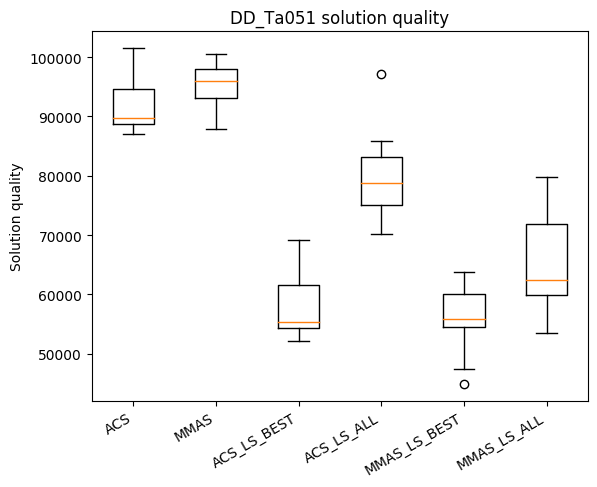
\includegraphics[width=1\linewidth]{plots/DD_Ta051__boxplot}
        \caption{Solution quality}
        \label{fig:ta_051:boxplot}
    \end{subfigure}
    \begin{subfigure}{.5\textwidth}
        \centering
        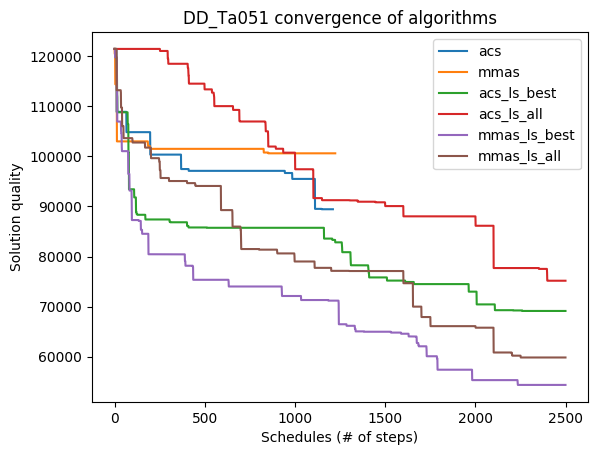
\includegraphics[width=1\linewidth]{plots/DD_Ta051__best_runs_convergence}
        \caption{Convergence of algorithms}
        \label{fig:ta_051:convergence}
    \end{subfigure}
    \caption{Boxplot and convergence for instance \texttt{Ta051}}
    \label{fig:ta_051}
\end{figure}

\begin{figure}[H]
    \begin{subfigure}{.5\textwidth}
        \centering
        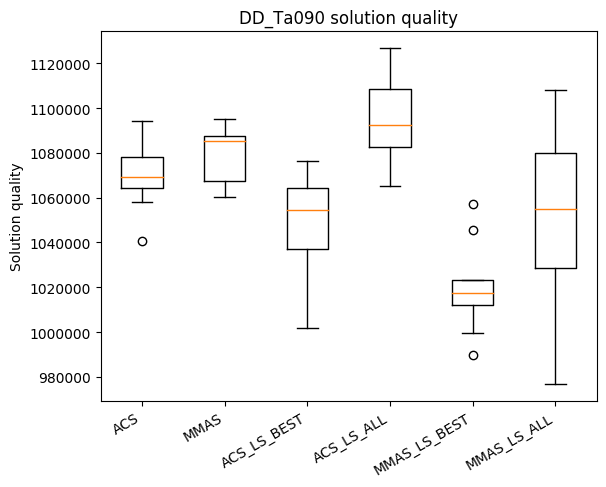
\includegraphics[width=1\linewidth]{plots/DD_Ta090__boxplot}
        \caption{Solution quality}
        \label{fig:ta_090:boxplot}
    \end{subfigure}
    \begin{subfigure}{.5\textwidth}
        \centering
        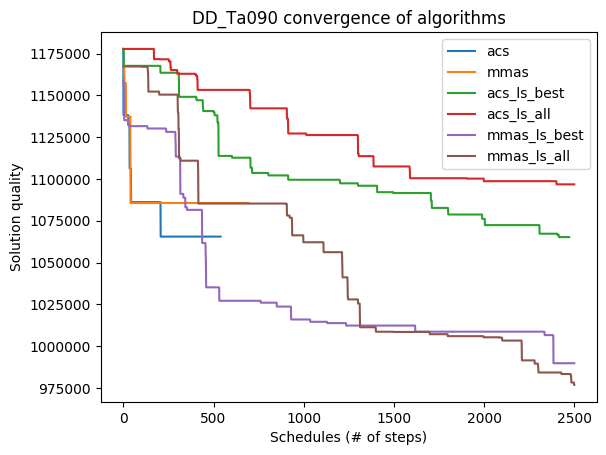
\includegraphics[width=1\linewidth]{plots/DD_Ta090__best_runs_convergence}
        \caption{Convergence of algorithms}
        \label{ig:ta_090:convergence}
    \end{subfigure}
    \caption{Boxplot and convergence for instance \texttt{Ta090}}
    \label{fig:ta_090}
\end{figure}

\section{Conclusion}


In this paper we describe the Permutation Flow Shop Problem with Weighted Tardiness minimization objective. We provided the implementation of two Ant Colony Optimization algorithms, ACS and MMAS, to solve the problem. Following the main implementation, we described two rather simple local search methods that significantly improve the solutions generated by the basic algorithms. One important result that the results highlighted is the importance of local search in those ACO algorithms. In the future, one might be interested in studying the impact of the parameters (only tuned with \texttt{irace} in this context) on the algorithms and the results for this problem.

\bibliographystyle{splncs04}
\bibliography{SWARM}

\end{document}
